\begin{frame}
	\frametitle{Projektverlauf\hfill{}\footnotesize \group}
	\framesubtitle{Visualisierung mit gource}
	\begin{columns}
		\begin{column}{0.5\textwidth}
			\begin{block}{Gerenderte Animation von github.com/accefa/doku}
				\movie[width=4cm,height=4cm, externalviewer]{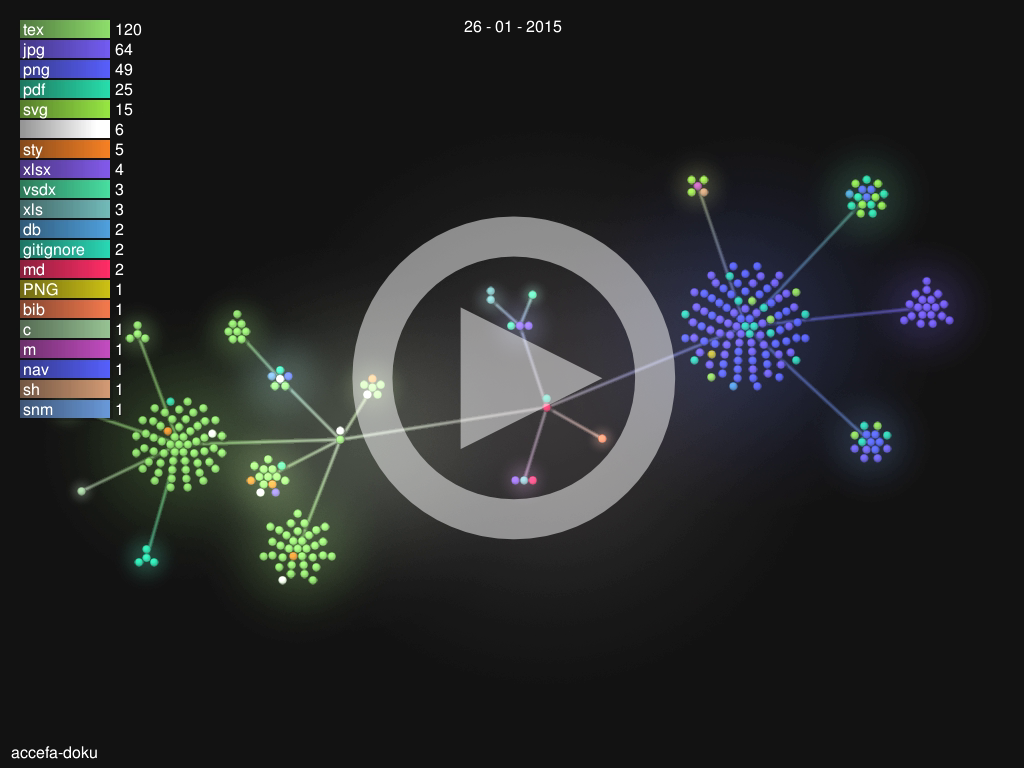
\includegraphics[width=1\textwidth]{../../fig/gource_play.png}}{gource-dark.mp4}
				\\ gource-dark.mp4 \hfill{} 1:24 min
			\end{block}
		\end{column}
		\begin{column}{0.5\textwidth}
			\begin{exampleblock}{gource Parameter}
				\lstinputlisting{gource-commands.txt}
			\end{exampleblock}
		\end{column}
	\end{columns}
\end{frame}
